\documentclass[10pt]{article}

\usepackage[paperwidth=210mm,paperheight=250mm,
  textwidth=200mm,textheight=244mm,top=3mm,left=5mm]{geometry}
\usepackage{amsmath,array,tabularx,tikz,xcolor}
\usetikzlibrary{arrows.meta,calc,positioning}
\pagestyle{empty}

\definecolor{accent}{HTML}{A51C30}
\definecolor{charcoal}{HTML}{242424}
\definecolor{softgray}{HTML}{F3F3F3}

\begin{document}
\centering
\hyphenpenalty=10000
\exhyphenpenalty=10000

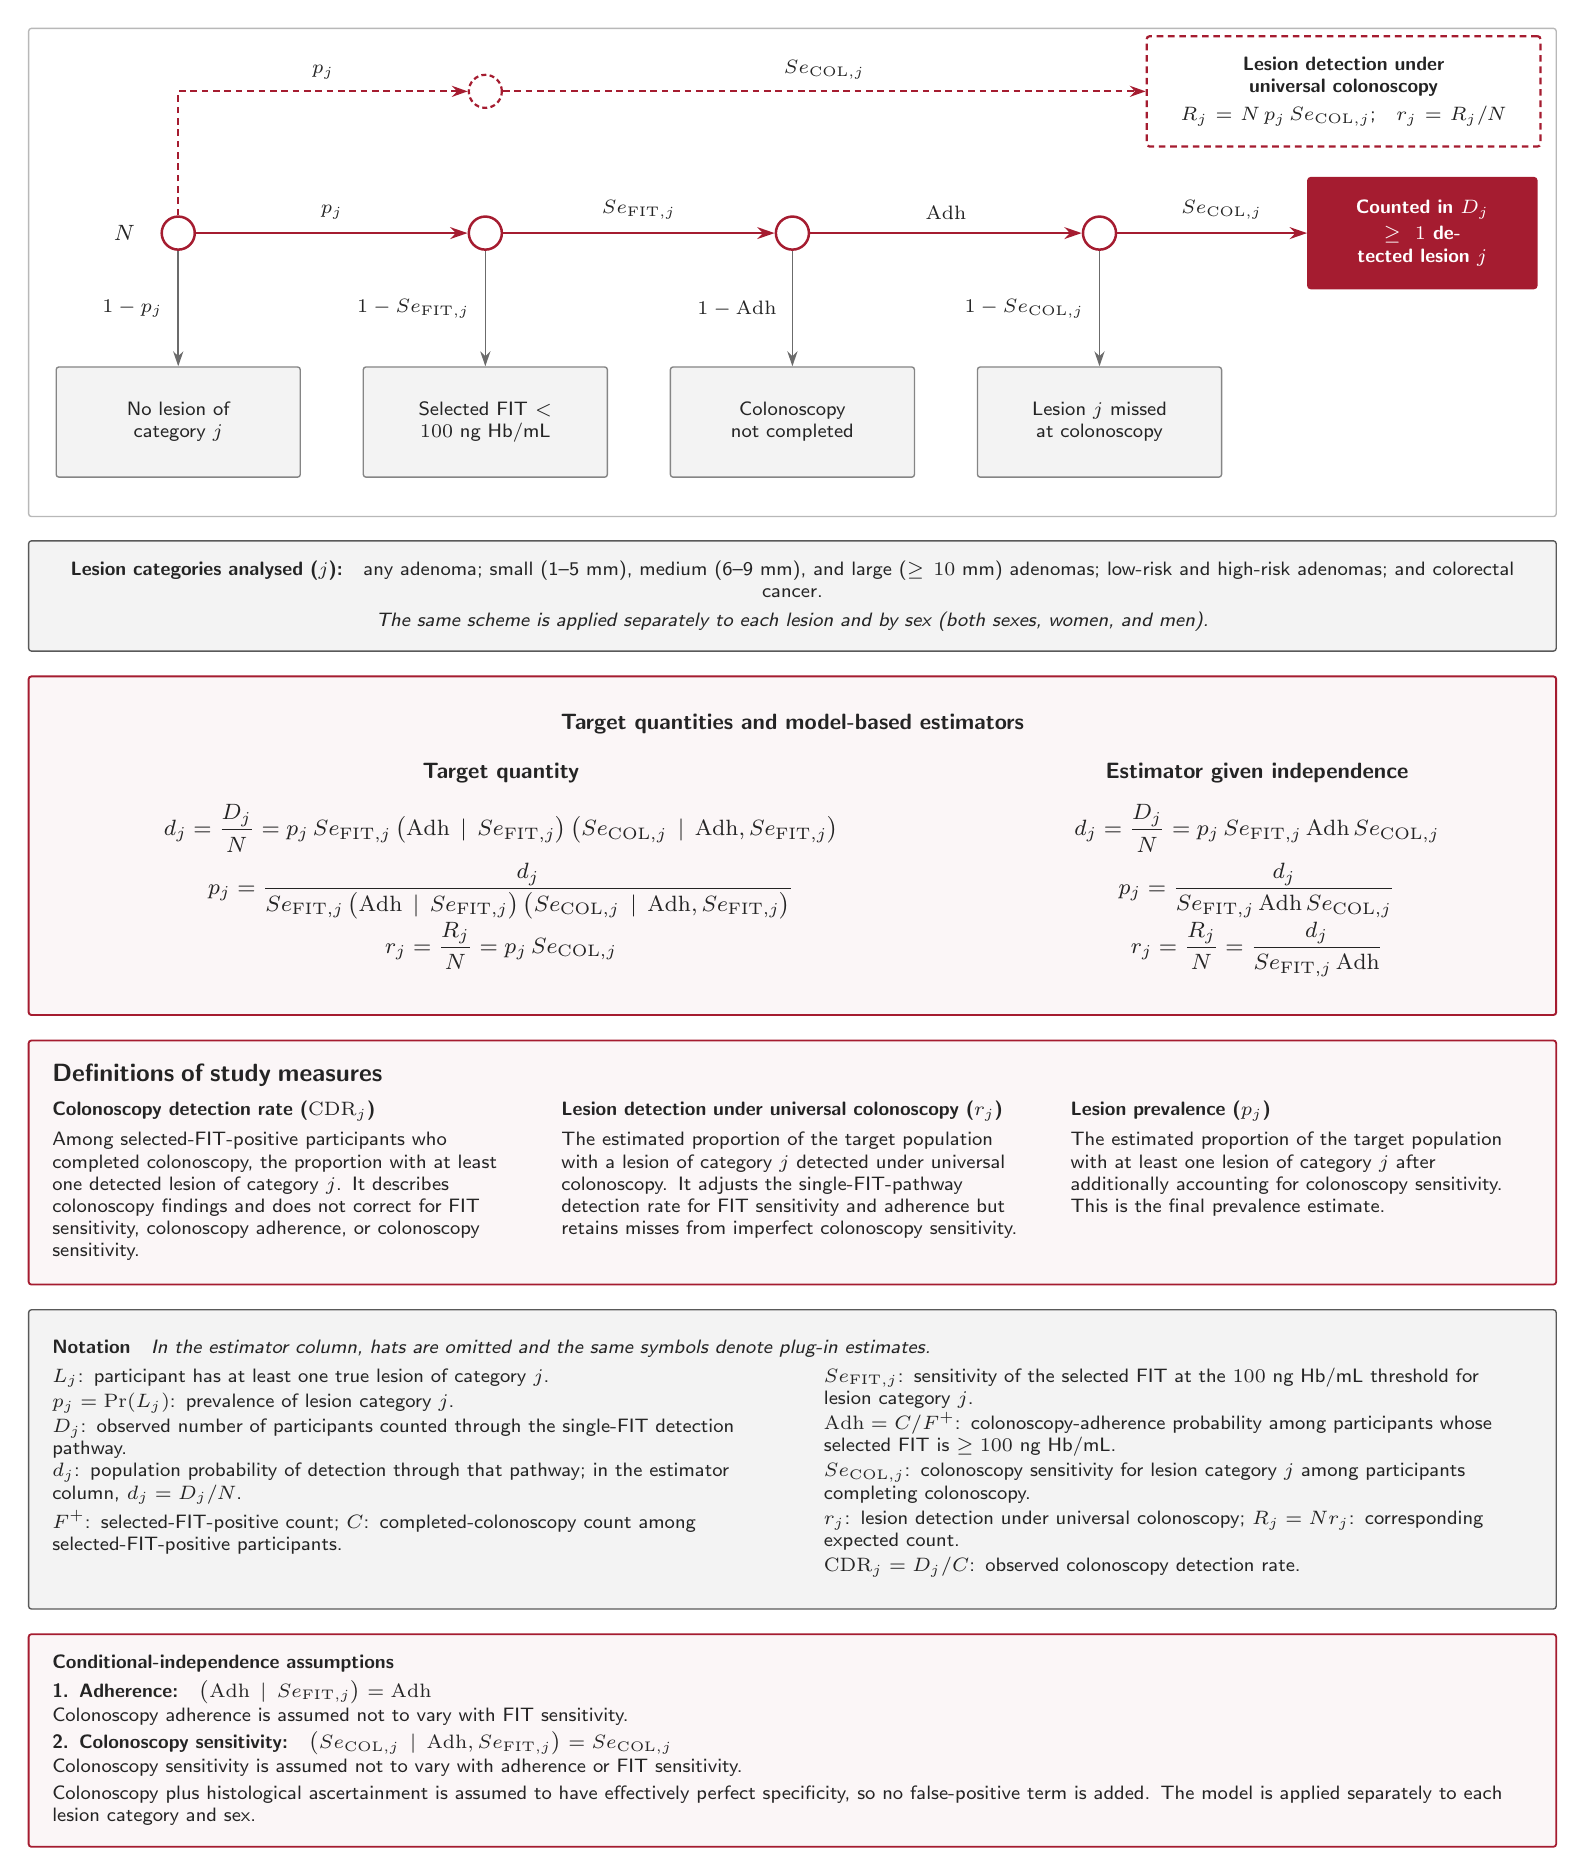
\begin{tikzpicture}[
  x=1mm,
  y=1mm,
  every node/.style={font=\sffamily, text=charcoal},
  mainarrow/.style={-{Stealth[length=2.2mm,width=1.5mm]},
    draw=accent, line width=0.95pt},
  counterarrow/.style={-{Stealth[length=2.0mm,width=1.4mm]},
    draw=accent, dashed, dash pattern=on 2.4pt off 1.7pt,
    line width=0.8pt},
  failarrow/.style={-{Stealth[length=1.9mm,width=1.3mm]},
    draw=black!58, line width=0.6pt},
  chance/.style={circle, draw=accent, fill=white, line width=0.9pt,
    minimum size=4.2mm, inner sep=0pt},
  counterchance/.style={circle, draw=accent, fill=white,
    dashed, dash pattern=on 1.8pt off 1.2pt, line width=0.8pt,
    minimum size=4.2mm, inner sep=0pt},
  terminal/.style={draw=black!48, fill=softgray, rounded corners=1pt,
    line width=0.5pt, text width=25mm, minimum width=31mm,
    minimum height=14mm, align=center, inner xsep=3mm, inner ysep=1.5mm,
    font=\sffamily\scriptsize},
  detected/.style={draw=accent, fill=accent, rounded corners=1pt,
    line width=0.8pt, text=white, text width=23mm, minimum width=29mm,
    minimum height=14mm, align=center, inner xsep=3mm, inner ysep=1.5mm,
    font=\sffamily\scriptsize\bfseries},
  counterterminal/.style={draw=accent, fill=white, rounded corners=1pt,
    dashed, dash pattern=on 2.4pt off 1.7pt, line width=0.8pt,
    text width=44mm, minimum width=50mm, minimum height=14mm,
    align=center, inner xsep=3mm, inner ysep=1.2mm,
    font=\sffamily\scriptsize},
  branchlabel/.style={align=center, font=\sffamily\scriptsize,
    fill=white, inner xsep=1.1mm, inner ysep=0.6mm},
  formulabox/.style={draw=accent, fill=accent!4, rounded corners=1pt,
    line width=0.7pt, text width=188mm, minimum width=194mm,
    minimum height=43mm, align=center, inner xsep=3mm, inner ysep=3mm,
    font=\sffamily\footnotesize},
  notation/.style={draw=black!65, fill=softgray, rounded corners=1pt,
    line width=0.5pt, text width=188mm, minimum width=194mm,
    minimum height=38mm, align=left, inner xsep=3mm, inner ysep=2mm,
    font=\sffamily\scriptsize},
  assumptions/.style={draw=accent, fill=accent!4, rounded corners=1pt,
    line width=0.65pt, text width=188mm, minimum width=194mm,
    minimum height=27mm, align=left, inner xsep=3mm, inner ysep=2mm,
    font=\sffamily\scriptsize},
  lesionbar/.style={draw=black!65, fill=softgray, rounded corners=1pt,
    line width=0.5pt, text width=188mm, minimum width=194mm,
    minimum height=14mm, align=center, inner xsep=3mm, inner ysep=1.0mm,
    font=\sffamily\scriptsize},
  definitions/.style={draw=accent, fill=accent!4, rounded corners=1pt,
    line width=0.65pt, text width=188mm, minimum width=194mm,
    minimum height=31mm, align=left, inner xsep=3mm, inner ysep=1.3mm,
    font=\sffamily\scriptsize}
]

\draw[black!28, rounded corners=1pt, line width=0.5pt]
  (-97,-5) rectangle (97,-67);

\node[chance] (root) at (-78,-31) {};
\node[chance] (lesion) at (-39,-31) {};
\node[chance] (fitpositive) at (0,-31) {};
\node[chance] (colonoscopy) at (39,-31) {};
\node[detected] (detected) at (80,-31)
  {Counted in $D_j$\\[0.5mm]
   $\geq1$ detected lesion $j$};

\node[anchor=east, font=\sffamily\footnotesize\bfseries]
  at ($(root.west)+(-2mm,0)$) {$N$};

\draw[mainarrow] (root) -- node[branchlabel, above=1.0mm] {%
  $p_j$} (lesion);
\draw[mainarrow] (lesion) -- node[branchlabel, above=1.0mm] {%
  $Se_{\mathrm{FIT},j}$} (fitpositive);
\draw[mainarrow] (fitpositive) -- node[branchlabel, above=1.0mm] {%
  $\mathrm{Adh}$} (colonoscopy);
\draw[mainarrow] (colonoscopy) --
  node[branchlabel, pos=0.55, above=1.0mm] {%
  $Se_{\mathrm{COL},j}$} (detected.west);

% Counterfactual pathway: universal colonoscopy, bypassing FIT and adherence.
\node[counterchance] (counterlesion) at (-39,-13) {};
\node[counterterminal] (countertarget) at (70,-13) {%
  {\bfseries Lesion detection under universal colonoscopy}\\[0.7mm]
  $R_j=N\,p_j\,Se_{\mathrm{COL},j}$;\quad $r_j=R_j/N$};
\draw[counterarrow] (root.north) -- (-78,-13) --
  node[branchlabel, above=0.8mm] {$p_j$} (counterlesion);
\draw[counterarrow] (counterlesion) --
  node[branchlabel, above=0.8mm] {$Se_{\mathrm{COL},j}$}
  (countertarget.west);

\node[terminal] (nolesion) at (-78,-55) {No lesion of category $j$};
\node[terminal] (fitnegative) at (-39,-55)
  {Selected FIT $<100$ ng Hb/mL};
\node[terminal] (nocolonoscopy) at (0,-55)
  {Colonoscopy not completed};
\node[terminal] (missed) at (39,-55)
  {Lesion $j$ missed at colonoscopy};

\draw[failarrow] (root) -- node[branchlabel, left=0.8mm] {$1-p_j$}
  (nolesion.north);
\draw[failarrow] (lesion) --
  node[branchlabel, left=0.8mm] {$1-Se_{\mathrm{FIT},j}$}
  (fitnegative.north);
\draw[failarrow] (fitpositive) --
  node[branchlabel, left=0.8mm] {$1-\mathrm{Adh}$}
  (nocolonoscopy.north);
\draw[failarrow] (colonoscopy) --
  node[branchlabel, left=0.8mm] {$1-Se_{\mathrm{COL},j}$}
  (missed.north);

% All full-width panels use the same 3 mm vertical gap.
\node[lesionbar, anchor=north] (lesions) at (0,-70) {%
  {\bfseries Lesion categories analysed ($j$):}\quad
  any adenoma; small (1--5 mm), medium (6--9 mm), and large
  ($\geq10$ mm) adenomas; low-risk and high-risk adenomas; and colorectal
  cancer.\\[0.8mm]
  {\slshape
  The same scheme is applied separately to each lesion and by sex
  (both sexes, women, and men).}
};

\node[formulabox, anchor=north] (factorisation)
  at ($(lesions.south)+(0,-3mm)$) {%
  {\bfseries Target quantities and model-based estimators}\\[1.0mm]
  \begingroup
  \renewcommand{\arraystretch}{1.85}%
  \begin{tabular}{@{}
    >{\centering\arraybackslash}p{114mm}
    @{\hspace{4mm}}
    >{\centering\arraybackslash}p{70mm}@{}}
    \textbf{Target quantity} & \textbf{Estimator given independence}\\[1.0mm]
    $\displaystyle d_j=\frac{D_j}{N}
      =p_j\,Se_{\mathrm{FIT},j}\,
      \bigl(\mathrm{Adh}\,\mid\,Se_{\mathrm{FIT},j}\bigr)\,
      \bigl(Se_{\mathrm{COL},j}\,\mid\,\mathrm{Adh},Se_{\mathrm{FIT},j}\bigr)$
    &
    $\displaystyle d_j=\frac{D_j}{N}
      =p_j\,Se_{\mathrm{FIT},j}\,\mathrm{Adh}\,Se_{\mathrm{COL},j}$\\[1.3mm]
    $\displaystyle p_j=
      \frac{d_j}{Se_{\mathrm{FIT},j}\,
      \bigl(\mathrm{Adh}\,\mid\,Se_{\mathrm{FIT},j}\bigr)\,
      \bigl(Se_{\mathrm{COL},j}\,\mid\,\mathrm{Adh},Se_{\mathrm{FIT},j}\bigr)}$
    &
    $\displaystyle p_j=
      \frac{d_j}
      {Se_{\mathrm{FIT},j}\,\mathrm{Adh}\,Se_{\mathrm{COL},j}}$\\[1.3mm]
    $\displaystyle r_j=\frac{R_j}{N}=p_j\,Se_{\mathrm{COL},j}$
    &
    $\displaystyle r_j=\frac{R_j}{N}
      =\frac{d_j}{Se_{\mathrm{FIT},j}\,\mathrm{Adh}}$
  \end{tabular}
  \endgroup
};

\node[definitions, anchor=north] (definitionsbox)
  at ($(factorisation.south)+(0,-3mm)$) {%
  {\small\bfseries Definitions of study measures}\\[1.4mm]
  \begin{tabularx}{\linewidth}{@{}X@{\hspace{6mm}}X@{\hspace{6mm}}X@{}}
  \begin{minipage}[t]{\linewidth}
  \raggedright
  \textbf{Colonoscopy detection rate ($\mathrm{CDR}_j$)}\\[1.0mm]
  Among selected-FIT-positive participants who completed colonoscopy, the
  proportion with at least one detected lesion of category $j$. It describes
  colonoscopy findings and does not correct for FIT sensitivity, colonoscopy
  adherence, or colonoscopy sensitivity.
  \end{minipage} &
  \begin{minipage}[t]{\linewidth}
  \raggedright
  \textbf{Lesion detection under universal colonoscopy ($r_j$)}\\[1.0mm]
  The estimated proportion of the target population with a lesion of category
  $j$ detected under universal colonoscopy. It adjusts the single-FIT-pathway
  detection rate for FIT sensitivity and adherence but retains misses from
  imperfect colonoscopy sensitivity.
  \end{minipage} &
  \begin{minipage}[t]{\linewidth}
  \raggedright
  \textbf{Lesion prevalence ($p_j$)}\\[1.0mm]
  The estimated proportion of the target population with at least one lesion
  of category $j$ after additionally accounting for colonoscopy sensitivity.
  This is the final prevalence estimate.
  \end{minipage}
  \end{tabularx}
};

\node[notation, anchor=north] (notationbox)
  at ($(definitionsbox.south)+(0,-3mm)$) {%
  {\bfseries Notation}\quad
  {\itshape In the estimator column, hats are omitted and the same symbols
  denote plug-in estimates.}\\[0.8mm]
  \begin{tabularx}{\linewidth}{@{}X@{\hspace{8mm}}X@{}}
  \raggedright
  $L_j$: participant has at least one true lesion of category $j$.\\[0.4mm]
  $p_j=\Pr(L_j)$: prevalence of lesion category $j$.\\[0.4mm]
  $D_j$: observed number of participants counted through the single-FIT
  detection pathway.\newline
  $d_j$: population probability of detection through that pathway; in the
  estimator column, $d_j=D_j/N$.\\[0.4mm]
  $F^+$: selected-FIT-positive count; $C$: completed-colonoscopy count among
  selected-FIT-positive participants.
  &
  \raggedright
  $Se_{\mathrm{FIT},j}$: sensitivity of the selected FIT at the
  $100$ ng Hb/mL threshold for lesion category $j$.\\[0.4mm]
  $\mathrm{Adh}=C/F^+$: colonoscopy-adherence probability among participants
  whose selected FIT is $\geq100$ ng Hb/mL.\\[0.4mm]
  $Se_{\mathrm{COL},j}$: colonoscopy sensitivity for lesion category $j$ among
  participants completing colonoscopy.\\[0.4mm]
  $r_j$: lesion detection under universal colonoscopy;
  $R_j=Nr_j$: corresponding expected count.\\[0.4mm]
  $\mathrm{CDR}_j=D_j/C$: observed colonoscopy detection rate.
  \end{tabularx}
};

\node[assumptions, anchor=north] (assumptionbox)
  at ($(notationbox.south)+(0,-3mm)$) {%
  {\bfseries Conditional-independence assumptions}\\[0.8mm]
  \textbf{1. Adherence:}\quad
  $\bigl(\mathrm{Adh}\,\mid\,Se_{\mathrm{FIT},j}\bigr)=\mathrm{Adh}$\\[0.3mm]
  Colonoscopy adherence is assumed not to vary with FIT sensitivity.\\[0.6mm]
  \textbf{2. Colonoscopy sensitivity:}\quad
  $\bigl(Se_{\mathrm{COL},j}\,\mid\,
  \mathrm{Adh},Se_{\mathrm{FIT},j}\bigr)=Se_{\mathrm{COL},j}$\\[0.3mm]
  Colonoscopy sensitivity is assumed not to vary with adherence or FIT
  sensitivity.\\[0.6mm]
  Colonoscopy plus histological ascertainment is assumed to have effectively
  perfect specificity, so no false-positive term is added. The model is applied
  separately to each lesion category and sex.
};

\end{tikzpicture}
\end{document}
